\documentclass{article}

% if you need to pass options to natbib, use, e.g.:
%     \PassOptionsToPackage{numbers, compress}{natbib}
% before loading neurips_2024


% ready for submission
\usepackage{MPL}
\usepackage{graphicx}

% to compile a preprint version, e.g., for submission to arXiv, add add the
% [preprint] option:
%     \usepackage[preprint]{neurips_2024}


% to compile a camera-ready version, add the [final] option, e.g.:
%     \usepackage[final]{neurips_2024}


% to avoid loading the natbib package, add option nonatbib:
%    \usepackage[nonatbib]{neurips_2024}


\usepackage[utf8]{inputenc} % allow utf-8 input
\usepackage[T1]{fontenc}    % use 8-bit T1 fonts
\usepackage{hyperref}       % hyperlinks
\usepackage{url}            % simple URL typesetting
\usepackage{booktabs}       % professional-quality tables
\usepackage{amsfonts}       % blackboard math symbols
\usepackage{nicefrac}       % compact symbols for 1/2, etc.
\usepackage{microtype}      % microtypography
\usepackage{xcolor}         % colors


\title{Driver Activity Detection}

% The \author macro works with any number of authors. There are two commands
% used to separate the names and addresses of multiple authors: \And and \AND.
%
% Using \And between authors leaves it to LaTeX to determine where to break the
% lines. Using \AND forces a line break at that point. So, if LaTeX puts 3 of 4
% authors names on the first line, and the last on the second line, try using
% \AND instead of \And before the third author name.


\author{%
  Shuvam Aich \\
  Department of Computer Science\\
  University of Stuttgart\\
  Stuttgart, Germany \\
  \texttt{---@stud.uni-stuttgart.de} \\
  \And
  Mugdha Asgekar \\
  Department of Computer Science\\
  University of Stuttgart\\
  Stuttgart, Germany \\
  \texttt{---@stud.uni-stuttgart.de} \\
  \AND
  Prateek Chaturvedi \\
  Department of Computer Science\\
  University of Stuttgart\\
  Stuttgart, Germany \\
  \texttt{---@stud.uni-stuttgart.de} \\
  \And
  Mahdi Jafarkhani \\
  Department of Computer Science\\
  University of Stuttgart\\
  Stuttgart, Germany \\
  \texttt{st186851@stud.uni-stuttgart.de} \\
}

\begin{document}

\maketitle


\begin{abstract}
  The abstract paragraph should be indented \nicefrac{1}{2}~inch (3~picas) on
  both the left- and right-hand margins. Use 10~point type, with a vertical
  spacing (leading) of 11~points.  The word \textbf{Abstract} must be centered,
  bold, and in point size 12. Two line spaces precede the abstract. The abstract
  must be limited to one paragraph.
\end{abstract}


\section{Introduction}

\section{Project Workflow}

\section{Dataset Overview}

\section{Sliding Window}

\section{Metrics}

\section{Neural Detection Model}
Manuel and Roitberg \cite{drive_and_act_2019_iccv} evaluated various models for fine-grained driver activity recognition using the DriveAndAct dataset. They tested different approaches, including CNN-based methods (like C3D, P3D ResNet, and I3D) and body pose-based methods. They found out that the Inflated 3D ConvNet (I3D), an extension of the Inception-v1 network with 3D convolutions, achieved the highest accuracy (69.57\% on Validation, and 63.64\% on test) among all tested models for recognizing fine-grained driver activities.
I3D also outperformed body pose-based methods, which were less effective in classifying actions despite incorporating spatial and temporal streams.
In atomic action unit classification, I3D performed best in recognizing actions (56.07\%) and objects (56.15\%), though body pose-based approaches were better at identifying locations (56.5\%).Although for cross-view action recognition, I3D models struggled with domain shifts, performing significantly worse when tested on unseen views.
\subsection{I3D Model}
The Two-Stream Inflated 3D ConvNet (I3D) \cite{carreira2018quovadisactionrecognition} is a deep learning model designed for video action recognition. It extends 2D convolutional neural networks (CNNs) into 3D by "inflating" their filters and pooling kernels to operate in both spatial and temporal dimensions. This allows the model to effectively capture motion patterns in videos (Figure \ref{fig:i3d}).
\subsubsection{Key Features of I3D}
\begin{itemize}
    \item \textbf{3D Convolutions}: Unlike traditional 2D CNNs that process images independently, I3D uses 3D convolutional layers to extract spatiotemporal features from videos.
    \item \textbf{Inflation from 2D Networks}: The model is based on the Inception-v1 architecture, with its 2D filters expanded into 3D. This allows it to reuse ImageNet pre-trained weights, improving efficiency and performance.
    \item \textbf{Two-Stream Configuration}: I3D processes both RGB frames (spatial information) and Optical flow (motion information). These two streams are trained separately and their outputs are fused at the end.
\end{itemize}

\begin{figure}[h]
    \centering
    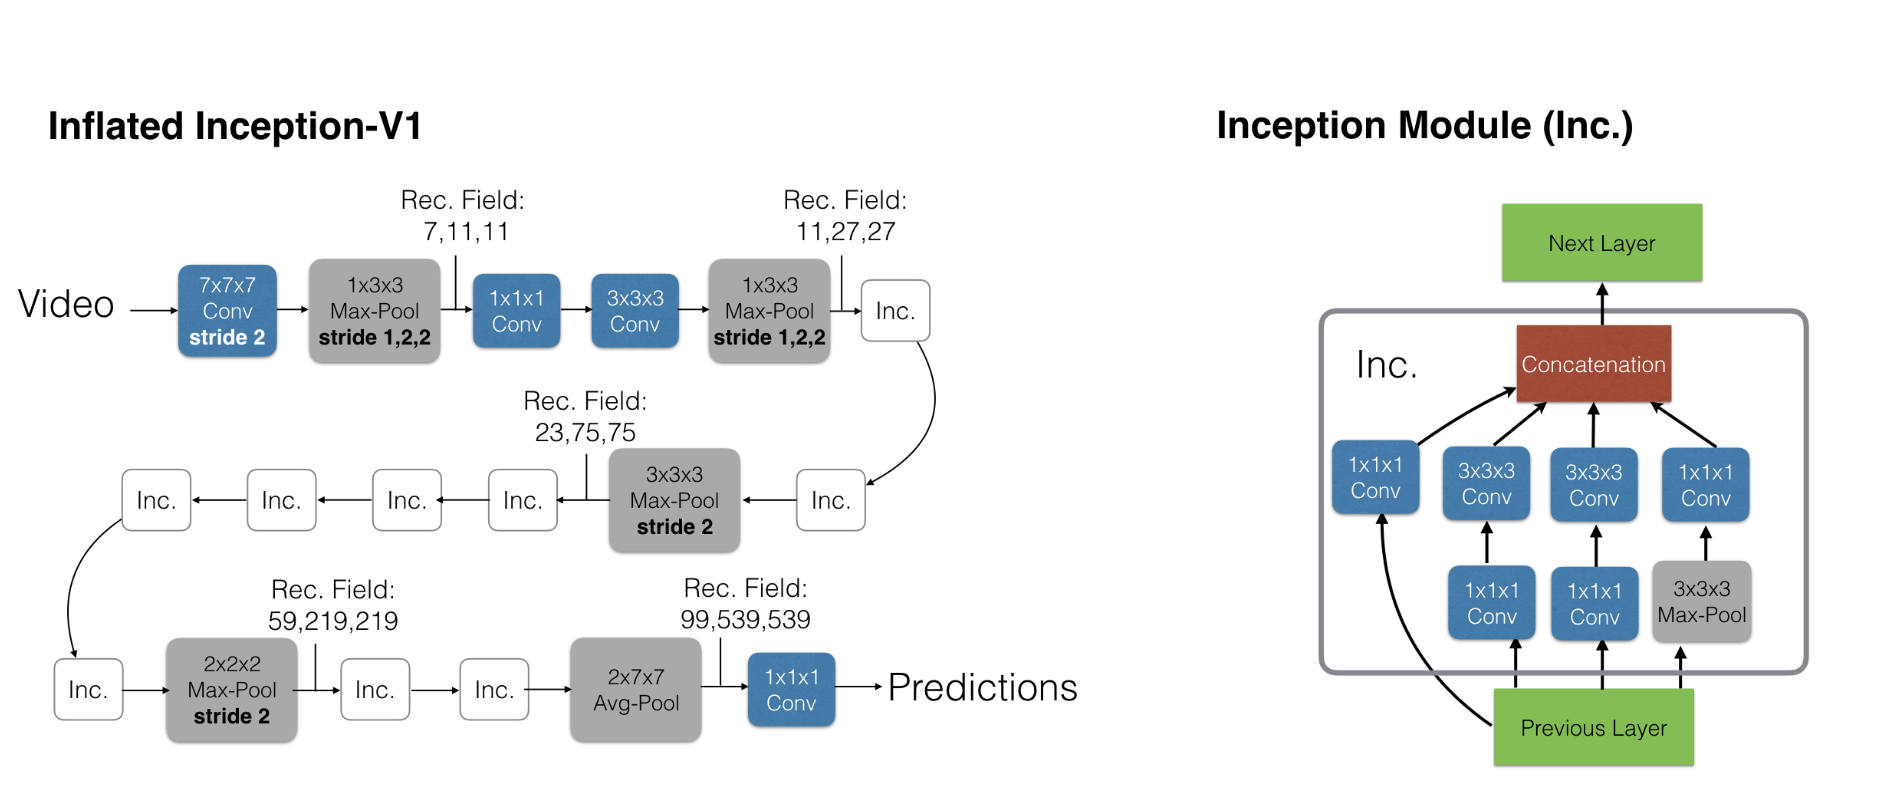
\includegraphics[width=0.8\linewidth]{figs/i3d.png}
    \caption{The Inflated Inception-V1 architecture (left) and its detailed inception submodule (right). The strides of convolution and pooling
operators are 1 where not specified, and batch normalization layers, ReLu’s and the softmax at the end are not shown. The theoretical
sizes of receptive field sizes for a few layers in the network are provided in the format “time,x,y” – the units are frames and pixels. The
predictions are obtained convolutionally in time and averaged.\cite{carreira2018quovadisactionrecognition}}
    \label{fig:i3d}
\end{figure}

\subsection{I3D Model as baseline model}
We utilized the I3D model for recognition in our project. We evaluated a pre-trained I3D model and performed inference on all videos in the Kinetic Color category. Figure \ref{fig:i3d-acc} illustrates the model's accuracy on the DriveAndAct dataset. The dataset includes 15 viewpoints, each comprising two runs, except for viewpoint 9, which lacked annotation for the second run. The average accuracy is 82.26\% for our baseline model.
We noticed the main reason for misclassfying each frame to its action is either by:
\begin{itemize}
    \item \textbf{Latency in Annotation}: Since human-labeled annotations (ground truths) lack a strict consensus on the exact start time of an action, some degree of misclassification is inevitable. In this context, misclassifying an action by at most 10 frames is considered acceptable or, in other words, irreducible.
    \item \textbf{Fast Switching Actions}: The model exhibited rapid transitions between actions, sometimes within less than 3 frames. This behavior was of particular interest to us, and we hypothesized that applying a neural network or transformer architecture on top of the I3D model could help reduce this misclassification.
\end{itemize}
\begin{figure}[h]
    \centering
    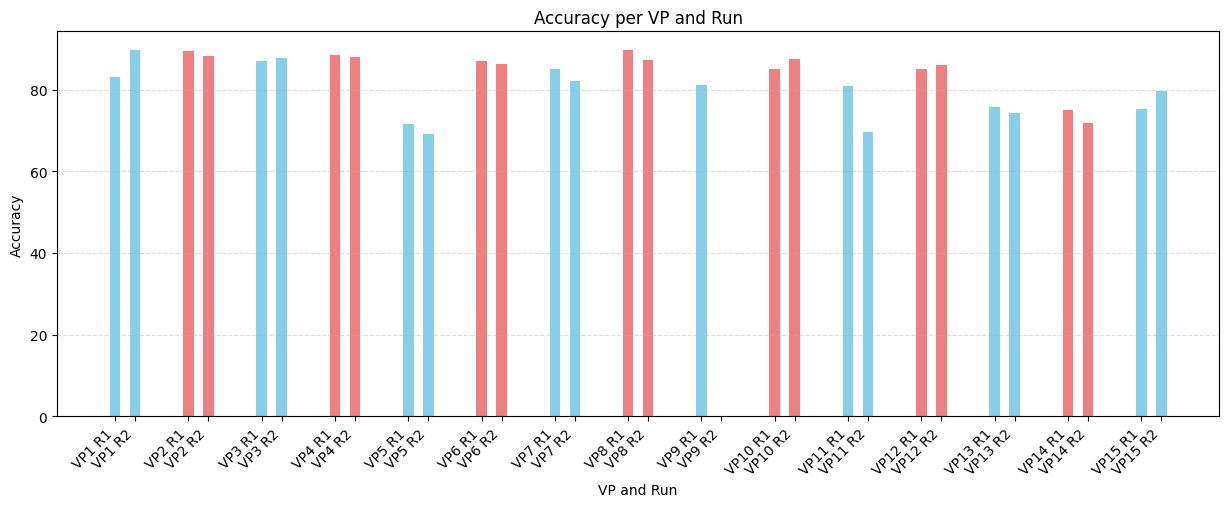
\includegraphics[width=0.8\linewidth]{i3d-acc.png}
    \caption{Accuracy for recognition task with I3D model on all viewpoints and runs on Kinetic Color category, DriveAndAct dataset}
    \label{fig:i3d-acc}
\end{figure}
\section{Conclusion}

\bibliographystyle{alpha}
\bibliography{MPL}

\end{document}